\documentclass[twocolumn]{article}
\usepackage{graphicx}
\usepackage{url}
\usepackage{amsmath}
\usepackage{amssymb}
\usepackage{amsfonts}
\usepackage{xcolor}
\usepackage{array}
\usepackage{colortbl}
\usepackage{float}
\usepackage{subcaption}
\usepackage{caption}
\usepackage{booktabs}
\usepackage{geometry}
\usepackage{multirow}
\usepackage{hyperref}
\geometry{margin=2.5cm}
\usepackage{authblk}
\usepackage{enumitem}
\usepackage{tikz}
\usetikzlibrary{shapes.geometric,arrows.meta,positioning,fit,backgrounds,calc}
\usepackage{algorithm}
\usepackage{algpseudocode}

%%
\title{CLAIP: Dual Corroboration and Segment-Aligned Contrastive Learning\\
for Domain Ontology Construction from Meeting Video, Toward Meeting Intelligence}

\author[1]{Takato Yasuno}
\author[1]{Atsuhiro Yamamoto}
\author[1]{Kazuki Izumi}
\affil[1]{Yachiyo Engineering Co., Ltd., Japan}
\affil[ ]{Email: yasunotkt@gmail.com}

\date{}

\begin{document}

%% English headings for abstract and references
\renewcommand{\abstractname}{Abstract}
\renewcommand{\refname}{References}
\renewcommand{\figurename}{Figure}
\renewcommand{\tablename}{Table}

\maketitle

%% ====================================================================
\begin{abstract}
%% ====================================================================

Specialized engineering organizations accumulate much of their domain expertise in recorded
design-review meeting video, yet this content rarely feeds back into a reusable, independently
verified domain ontology. We pursue this capability -- deriving and corroborating structured
domain knowledge directly from a meeting's own audio, screen-share, and speech content, toward what
we call \emph{Meeting Intelligence} -- using a bridge-repair design-review meeting as a concrete
case study. Prior work on domain-dictionary correction for Japanese construction-meeting ASR took a
first step in this direction, corroborating candidate terms against a single, independently
verified source -- a static damage-cause ontology -- mined either in bulk or from the meeting's own
corrected audio transcript \emph{after} speech recognition had already run. This paper extends that
pipeline with a second, independent
corroboration source available \emph{before} speech recognition runs: optical character recognition
(OCR) and image captioning applied to video frames sampled from the meeting's own screen-share
content (slides, sticky-note review comments), merged into the domain dictionary so that the
automatic speech recognizer's own vocabulary bias already reflects what was visibly written on
screen. We further build a shared three-modality (audio, image, text) embedding space via
contrastive (CLAIP-style) projection-head training over the meeting's own utterance-aligned data, as
a first step toward cross-modal meeting search. We compare two frame-sampling strategies for this
image branch on a real 44.9-minute Google Meet recording (914 transcribed utterances, 6 speakers):
fixed 10-second-interval sampling and diarization-utterance-segment-driven dense sampling. Under a
controlled, fixed-reference-vocabulary evaluation, segment-driven sampling nearly triples kept,
de-duplicated frames (92 to 264) and improves candidate-term coverage by 69\% (55 to 93 terms, 42
entirely new), while guaranteeing at least one contrastive training triple per transcribed
utterance and increasing total triples more than tenfold (90 to 961; all 914 utterances covered, 43
contributing more than one triple because the shared screen changed mid-utterance). This denser,
utterance-aligned training data also nearly doubles a qualitative cross-modal retrieval sanity
check (2/7 to 4/7 known domain terms correctly retrieved). We additionally report two previously
unreported OCR-specific candidate-extraction failure modes -- reviewer-name/content concatenation
and adjacent sticky-note text duplication -- with lightweight, non-LLM mitigations, and an empirical
training-stability finding: increasing contrastive-triple count by an order of magnitude induces
late-training loss instability under fixed-learning-rate, full-batch Adam, mitigated here by
best-checkpoint retention. Motivated by a specific failure case -- a Google Meet standby tile
(black background, centered name/photo) entering a triple in place of genuine shared-screen
content, which should weaken the image-paired losses while leaving the audio-text pair unaffected --
we introduce a per-modality-pair loss-weighting hyperparameter and test one hand-chosen setting
(down-weighting the two image-paired terms, up-weighting audio-text) in a seed-matched controlled
comparison: it sharpens the audio-text pair by 19.8\% (rescored on a common, unweighted basis)
without measurably degrading either image-paired term, reduces the number of late-training loss
spikes from two to one, and leaves the 7-query retrieval hit rate unchanged (4/7), suggesting the
weighting is a safe, if modest, refinement rather than a generalizable fix. We report all results
candidly as a single-video case study: the retrieval numbers are a qualitative proof of concept, not
a statistically validated benchmark. Taken
together, these results are a concrete, if preliminary, step toward Meeting Intelligence: showing
that a single bridge-repair design-review recording's own video and audio can already corroborate
and expand a verified domain ontology, a mechanism we intend to generalize across construction's
other specialized engineering departments in future work.

\end{abstract}

\noindent
\textbf{Keywords:} Automatic Speech Recognition, Multimodal Corroboration, Contrastive
Representation Learning, Optical Character Recognition, Domain Dictionary Correction, Speaker
Diarization, Ontology Construction, Meeting Intelligence.

%% ====================================================================
\section{Introduction}
\label{sec:intro}
%% ====================================================================

\subsection{Background and Motivation}

Infrastructure-engineering organizations hold much of their domain expertise not in written
documents but in the spoken and visually shared content of recorded design-review meetings --
videos that are rarely mined back into a reusable, verified domain ontology once the meeting ends.
This paper's overarching goal is \emph{Meeting Intelligence}: constructing and continuously
corroborating a specialized-domain ontology directly from an organization's own meeting video, using
a real bridge-repair external design-review recording as our concrete case study throughout.

A companion paper~\cite{yasuno2026meetingasr} (hereafter, \emph{the base paper}) presented an
on-premise pipeline for Japanese construction-meeting speech recognition that corrects
domain-specific vocabulary errors via a morphology-aware, two-pass dictionary-correction algorithm,
and expands that dictionary's coverage by corroborating candidate terms against an independently
verified damage-cause ontology~\cite{yasuno2026ontology}, either in bulk (meeting-independent) or
per-meeting, by mining the pipeline's own corrected transcript \emph{after} automatic speech
recognition (ASR) has already run. That paper's own concluding future work identified audio-visual
capture (Microsoft Teams, Google Meet, Zoom) as an open engineering direction, and noted that the
raw ASR transcript alone under-exploits the lived engineering experience voiced in review meetings.

Construction-design review meetings, however, are rarely audio-only in substance: participants
routinely share their screen to walk through design drawings, inspection photographs, and
document-viewer sessions annotated with stacked sticky-note review comments, each naming a specific
structural member, damage mode, or repair method in written form. This visual channel is a second,
independent source of exactly the domain vocabulary that the base paper's dictionary-correction
algorithm is trying to recover from audio alone -- and, critically, this visual content is available
to the pipeline \emph{before} ASR is run on a given recording, unlike the base paper's per-meeting
audio-side extraction, which is necessarily post-hoc. This paper designs and evaluates a
mechanism that corroborates candidate terms using this screen-share content, merges it into the
dictionary before ASR runs, and, following the project's own Concept Note's CLAIP
(Contrastive Language-Audio-Image Pre-training) vision, projects audio, image, and text
representations of the meeting into one shared embedding space via contrastive learning, as a
foundation for future cross-modal meeting search.

\subsection{Problem Statement and Challenges}

Extending dictionary corroboration and contrastive representation learning to a meeting's own
screen-share frames raises three challenges addressed in this paper: (a) how densely frames should
be sampled from the source video -- a fixed wall-clock interval is simple but samples independently
of the speech it will be aligned with, and may both miss slide transitions that happen between
sample points and over-sample long stretches of an unchanging slide; (b) OCR text extracted from a
screenshot of stacked review comments has none of natural language's word-boundary and
particle/honorific cues that the base paper's audio-side candidate-extraction mitigations rely on,
so OCR-specific candidate-extraction failure modes must be identified and mitigated on their own
terms; and (c) aligning each transcribed utterance with the frame(s) shown while it was spoken, and
training a shared embedding space over the resulting (image, audio, text) triples, must both
guarantee adequate training-data density and remain numerically stable as that density grows by an
order of magnitude.

\subsection{Contributions}

This paper makes the following contributions:
\begin{enumerate}[leftmargin=*,itemsep=1pt]
  \item \textbf{Dual corroboration.} We extend the base paper's ontology-corroboration
    dictionary-expansion mechanism with a second, independent in-meeting evidence source --
    screen-share frame OCR -- merged into the dictionary \emph{before} ASR executes, so the
    recognizer's own vocabulary bias (its \texttt{initial\_prompt}) already reflects what was
    visibly written on screen, unlike the base paper's audio-side per-meeting mechanism, which is
    necessarily post-hoc.
  \item \textbf{A controlled comparison of two frame-sampling strategies.} We compare fixed
    10-second-interval sampling against diarization-utterance-segment-driven dense sampling under a
    fixed-reference-vocabulary evaluation designed specifically to isolate the sampling method's
    effect from confounding dictionary-state differences, finding the latter improves candidate-term
    coverage by 69\% (55 to 93 of 183 reference terms, 42 entirely new) and nearly triples kept,
    de-duplicated frames (92 to 264).
  \item \textbf{A segment-centric contrastive-triple construction algorithm} that guarantees at
    least one (image, audio, text) training triple per transcribed utterance (914/914 covered) and
    one additional triple for each distinct image shown if the shared screen changed mid-utterance
    (43 utterances), replacing a looser frame-centric, time-window heuristic and increasing total
    training triples more than tenfold (90 to 961).
  \item \textbf{Two previously unreported OCR-specific candidate-extraction failure modes} --
    reviewer-name/content concatenation and adjacent sticky-note text duplication, both arising from
    OCR text's lack of natural-language word-boundary cues -- together with lightweight,
    part-of-speech-based and string-level mitigations validated on real extracted candidates.
  \item \textbf{An empirical contrastive-training-stability finding}: scaling triple count by an
    order of magnitude (90 to 961) induces late-training loss instability under fixed-learning-rate,
    full-batch Adam optimization of InfoNCE projection heads, which we mitigate with best-checkpoint
    retention rather than learning-rate scheduling, reported as an engineering finding for
    small-scale, single-recording contrastive learning.
  \item \textbf{A qualitative cross-modal retrieval case study}, reported candidly as a
    single-video proof of concept rather than a statistically validated benchmark, showing the
    segment-centric design nearly doubles a 7-query sanity-check hit rate (2/7 to 4/7) against known
    high-confidence domain terms.
  \item \textbf{A per-modality-pair loss-weighting ablation} motivated by the standby-frame case
    (\S\ref{sec:method-training}): in a seed-matched controlled comparison, down-weighting the
    image-paired InfoNCE terms and up-weighting the audio-text term sharpens the audio-text pair by
    19.8\% without degrading either image-paired term, halves the observed late-training loss-spike
    count, and leaves the retrieval hit rate unchanged -- evidence, on this single recording and
    seed, that the weighting is a safe refinement rather than a generalizable fix.
\end{enumerate}

\subsection{Paper Organization}

\S\ref{sec:related} surveys related work in cross-modal contrastive pretraining, document/slide OCR,
multilingual text embeddings, and ontology construction and Meeting Intelligence, and positions this
paper relative to the base paper. \S\ref{sec:formulation} extends the base
paper's pipeline formalization with the image branch and the shared embedding space.
\S\ref{sec:method} details the methodology. \S\ref{sec:setup} and \S\ref{sec:results} report the
experimental setup and results. \S\ref{sec:discussion} discusses implications and limitations, and
\S\ref{sec:conclusion} concludes.

%% ====================================================================
\section{Related Work}
\label{sec:related}
%% ====================================================================

\subsection{Cross-Modal Contrastive Pretraining}

CLIP~\cite{radford2021clip} established that a shared embedding space between image and text
encoders, trained with a symmetric InfoNCE contrastive objective~\cite{oord2018cpc} over large-scale
noisy image-text pairs, enables strong zero-shot transfer; CLAP~\cite{elizalde2023clap} applies the
same recipe to audio-text pairs. The CLAIP design explored in this paper -- jointly projecting
audio, image, and text representations of the \emph{same} meeting into one space -- combines both
lines of work into three bilinear objectives (image-text, audio-text, image-audio) over a single
recording's own utterance-aligned data, rather than a large external paired corpus; we discuss the
resulting small-sample regime's distinct optimization behavior in \S\ref{sec:discuss-training}.
BLIP~\cite{li2022blip} generates natural-language image captions via a vision-language
encoder-decoder, which we use (\S\ref{sec:method}) for frames whose dominant content is a
photograph or diagram rather than a document screenshot; rinna's Japanese CLIP release, based on a
ViT-B/16 image encoder and a 12-layer Japanese text encoder~\cite{sawada2024release}, provides the
domain-appropriate (Japanese-capable) image-text branch of our shared space.

\subsection{Document and Slide OCR}

EasyOCR~\cite{jaided2020easyocr} combines a CRAFT-style text-detection network with a CRNN-style
recognizer, supporting Japanese and over 80 other languages without requiring a separately installed
native binary (unlike Tesseract) or a heavier deep-learning framework dependency beyond
PyTorch (unlike PaddleOCR, which we considered and rejected, \S\ref{sec:method}). Unlike the
general-purpose image captioning of \S\ref{sec:related}'s preceding subsection, OCR targets the
\emph{exact} written characters on screen, which matters directly for our setting: a design-review
sticky note reading a specific structural-member name is a much stronger domain-vocabulary signal
than a natural-language scene description of the same screenshot (\S\ref{sec:method}).

\subsection{Multilingual Text Embeddings}

For the text branch of the shared embedding space, we use multilingual-E5~\cite{wang2024e5}, a
Sentence-BERT-family~\cite{reimers2019sentencebert} embedding model trained with weakly-supervised
contrastive pretraining across 100+ languages, via the \texttt{sentence-transformers} library,
chosen for its balance of Japanese-language coverage and parameter count (base, not large) relative
to the 16\,GB consumer-GPU budget shared with the other encoders in our stack
(\S\ref{sec:setup}).

\subsection{Ontology Construction and Meeting Intelligence}

Classical ontology learning from text progressed from shallow, pattern- and statistics-based
term/relation extraction to deep-learning sequence models~\cite{al-aswadi2020ontology}, and more
recently to large-language-model-driven extraction, schema induction, and knowledge
fusion~\cite{du2024ontologyllm,bian2025llmkg}; multimodal knowledge-graph construction further fuses
image, text, and other modalities into a single graph~\cite{chen2023multimodalkg}. Enterprise-focused
work applies this machinery directly to organizational communication: an LLM-driven, activity-centric
knowledge graph unifying emails, calendars, chats, and meeting-preparation artifacts for expertise
discovery and analytics~\cite{kumar2025llmkgenterprise}, and a real-world multimodal meeting dataset
and benchmark for long-form transcription and summarization that fuses speech, vision, and text
cues~\cite{hangchen2025misp}, both of which we take as evidence that \emph{Meeting Intelligence} --
deriving reusable, structured domain knowledge directly from an organization's own recorded meetings
-- is an active and recognized goal distinct from meeting summarization alone. Unlike these text- or
synthetic-corpus-centric knowledge-graph-construction pipelines, this paper corroborates a narrow,
hand-verified domain dictionary directly from a single meeting's own screen-share and audio content,
trading construction generality for verifiability on exactly the vocabulary a design-review team
actually used.

\subsection{Positioning}

This paper is a direct methodological extension of the base paper~\cite{yasuno2026meetingasr}, which
remains the source of the underlying speaker-diarization, ASR, and morphology-aware
dictionary-correction mechanisms (\S\ref{sec:method} reuses its Algorithm~1 and dictionary-expansion
equation unchanged). We do not re-evaluate those base mechanisms here; this
paper's contribution is the new image branch, dual corroboration, and the CLAIP shared embedding
space layered on top, evaluated on the same case-study recording the base paper designates M9.

%% ====================================================================
\section{Problem Formulation}
\label{sec:formulation}
%% ====================================================================

We adopt the base paper's notation unchanged (preprocessing $p$, diarization $D$, segment-wise ASR
$T$, domain-dictionary correction $C_\varphi$, and the dictionary-expansion operators
$E_{\text{ont}}$, $E_{\text{meet}}$ defined there), and extend its dictionary-expansion equation
($\varphi \leftarrow \varphi_0 \cup \varphi_{\text{ont}} \cup \varphi_{\text{meet}}(g_{\varphi_0}(a))$)
with one additional expansion operator and a parallel shared-embedding-space formalization.

\textbf{Frame extraction.} Let $F(a) \rightarrow \{f_1,\dots,f_P\}$ denote a sampling function that
extracts a set of video frames from the raw recording $a$, each $f_p$ carrying a timestamp
$\mathrm{ts}(f_p)$. We study two instantiations of $F$ in this paper: $F_{\text{int}}$, which
samples at a fixed wall-clock interval independent of $D(w)$, and $F_{\text{seg}}$, which samples
one or more frames per diarization segment in $D_{\text{excl}}(w)$ (\S\ref{sec:method}). Critically,
both instantiations depend only on $a$ (and, for $F_{\text{seg}}$, on the audio-only diarization
$D_{\text{excl}}(w)$) -- neither depends on the ASR output $T(\cdot)$ -- so $F(a)$ is always
computable \emph{before} segment-wise ASR runs.

\textbf{De-duplication and resolution.} A perceptual-hash de-duplication pass
$\mathrm{dedup}(\{f_p\}) \rightarrow \{(f_p, \mathrm{kept}_p, \rho_p)\}$ marks each frame
$\mathrm{kept}_p \in \{0,1\}$ and assigns a \emph{represents} pointer $\rho_p$: $\rho_p = p$ if
$\mathrm{kept}_p = 1$, otherwise $\rho_p$ is the index of the nearest preceding kept frame with the
same (unchanged) visible content. Only kept frames are passed to OCR and captioning
(\S\ref{sec:method}); $\rho_p$ lets every candidate frame, kept or not, be resolved back to the one
frame whose text was actually extracted.

\textbf{OCR and captioning.} $O(f_p) \rightarrow x^{\text{ocr}}_p$ and $\mathrm{Cap}(f_p) \rightarrow
x^{\text{cap}}_p$ extract on-screen text and a natural-language caption, respectively, for each kept
frame; their concatenation $x_p \triangleq x^{\text{ocr}}_p \,\|\, x^{\text{cap}}_p$ is this frame's
\emph{unified semantic text}.

\textbf{Frame-derived vocabulary expansion.} Analogously to $E_{\text{ont}}$, we define
$E_{\text{frame}}\big(\{x^{\text{ocr}}_p\}\big) \rightarrow \varphi_{\text{frame}}$, which mines the
kept frames' OCR text for candidate terms via the same SudachiPy segmentation as
$E_{\text{ont}}/E_{\text{meet}}$ (\S\ref{sec:method}), classifies their relevance with the local LLM
exactly as $E_{\text{meet}}$ does (unlike $E_{\text{ont}}$'s candidates, a term appearing on one
meeting's own screen is not already confirmed domain vocabulary by construction), and corroborates
each candidate's resolved canonical $\hat{m}$ against \emph{both} independently verified sources:
\begin{equation}
  \mathrm{corrob}(m) \triangleq \mathbb{1}\big[\hat{m} \in \mathrm{dom}(\varphi_{\text{ont}}) \cup
    \mathrm{dom}(\varphi_{\text{frame}})\big],
  \label{eq:dual-corrob}
\end{equation}
recording which source(s) fired, $\mathrm{src}(m) \in \{\text{ont}, \text{frame}, \text{both},
\emptyset\}$, generalizing the base paper's single-source Equation~(corrob) to this paper's
\emph{dual} corroboration. The dictionary used by a given run becomes
\begin{equation}
  \varphi \leftarrow \varphi_0 \cup \varphi_{\text{ont}} \cup \varphi_{\text{frame}}\big(F(a)\big)
    \cup \varphi_{\text{meet}}\big(g_{\varphi'}(a)\big),
  \label{eq:expansion-frame}
\end{equation}
where $\varphi' \triangleq \varphi_0 \cup \varphi_{\text{ont}} \cup \varphi_{\text{frame}}(F(a))$.
Because $\varphi_{\text{frame}}$ depends only on $F(a)$, it is available before $g_{\varphi'}(a)$
(hence before $T(\cdot)$) is computed, letting the newly discovered screen-share vocabulary bias
Whisper's own \texttt{initial\_prompt} \emph{within the same pipeline run} -- the central
distinction from $\varphi_{\text{meet}}$, which can only ever expand the dictionary for a
\emph{future} run on the same recording.

\textbf{Shared embedding space.} Let $f_{\text{img}}, f_{\text{aud}}, f_{\text{txt}}$ be frozen,
pretrained encoders (\S\ref{sec:method}) mapping a kept frame, an audio segment, and a text string to
fixed-size embeddings, respectively. For a set of $N$ aligned triples
$\{(f_{\text{img}}(\cdot), f_{\text{aud}}(\cdot), f_{\text{txt}}(\cdot))_i\}_{i=1}^N$
(\S\ref{sec:method} defines two alignment strategies, frame-centric and segment-centric), three
learned linear projection heads $\pi_{\text{img}}, \pi_{\text{aud}}, \pi_{\text{txt}}: \mathbb{R}^{d_k}
\rightarrow \mathbb{R}^{d}$ are trained to maximize agreement between L2-normalized projections of
matched pairs via a symmetric InfoNCE objective (Equation~\ref{eq:infonce}, \S\ref{sec:method}),
summed over all three modality pairs. We study how the construction of the triple set $N$ -- in
particular, whether it is built per-frame or per-utterance-segment -- affects both $N$'s size and
the trained space's cross-modal retrieval quality (\S\ref{sec:results}).

%% ====================================================================
\section{Methodology}
\label{sec:method}
%% ====================================================================

\subsection{System Architecture}

Figure~\ref{fig:pipeline2} extends the base paper's pipeline (its Figure~1) with the image branch
and shared-embedding stages introduced in this paper. The image branch runs in a separate Python
virtual environment from the audio/dictionary branch (\S\ref{sec:setup}), orchestrated via
subprocess calls so GPU memory for each stage's models can be released before the next stage loads
(the same resource-management discipline the base paper applies across diarization and ASR).

\begin{figure}[t]
\centering
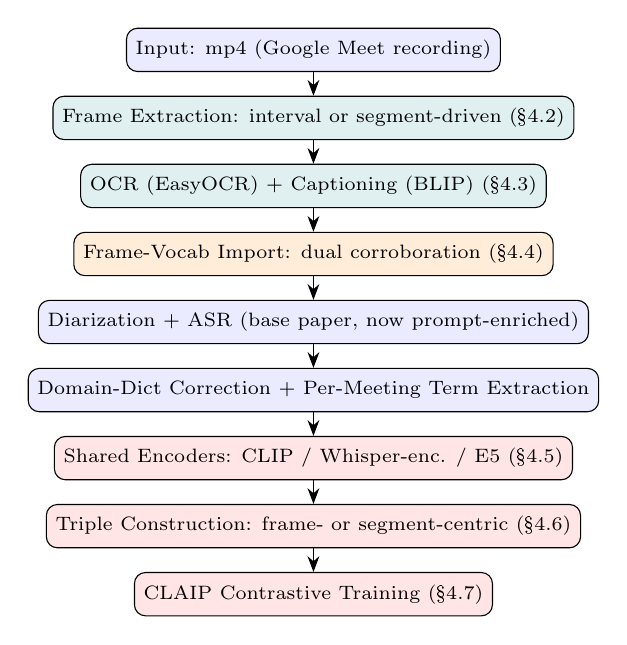
\begin{tikzpicture}[
  node distance=0.3cm,
  box/.style={draw, rounded corners, fill=blue!8, minimum width=4.0cm, minimum height=0.55cm, align=center, font=\scriptsize},
  img/.style={draw, rounded corners, fill=teal!12, minimum width=4.0cm, minimum height=0.55cm, align=center, font=\scriptsize},
  hl/.style={draw, rounded corners, fill=orange!15, minimum width=4.0cm, minimum height=0.55cm, align=center, font=\scriptsize},
  hl2/.style={draw, rounded corners, fill=red!10, minimum width=4.0cm, minimum height=0.55cm, align=center, font=\scriptsize},
  arr/.style={-{Stealth[length=2mm]}}
]
\node[box] (v0) {Input: mp4 (Google Meet recording)};
\node[img, below=of v0] (v1) {Frame Extraction: interval or segment-driven (\S4.2)};
\node[img, below=of v1] (v2) {OCR (EasyOCR) + Captioning (BLIP) (\S4.3)};
\node[hl, below=of v2] (v3) {Frame-Vocab Import: dual corroboration (\S4.4)};
\node[box, below=of v3] (v4) {Diarization + ASR (base paper, now prompt-enriched)};
\node[box, below=of v4] (v5) {Domain-Dict Correction + Per-Meeting Term Extraction};
\node[hl2, below=of v5] (v6) {Shared Encoders: CLIP / Whisper-enc. / E5 (\S4.5)};
\node[hl2, below=of v6] (v7) {Triple Construction: frame- or segment-centric (\S4.6)};
\node[hl2, below=of v7] (v8) {CLAIP Contrastive Training (\S4.7)};
\foreach \i/\j in {v0/v1,v1/v2,v2/v3,v3/v4,v4/v5,v5/v6,v6/v7,v7/v8}
  \draw[arr] (\i) -- (\j);
\end{tikzpicture}
\caption{Extended pipeline architecture. Teal stages (image branch) run in a separate Python
environment from the base paper's audio/dictionary stages (blue); orange/red stages (dual
corroboration, shared embeddings, contrastive training) are this paper's central contribution.
The frame-vocab import stage (\S4.4) re-enriches the dictionary \emph{before} diarization/ASR runs,
closing the same within-run dictionary-expansion loop the base paper describes
(Equation~\ref{eq:expansion-frame}) but from the image branch.}
\label{fig:pipeline2}
\end{figure}

\subsection{Screen-Share Frame Extraction}
\label{sec:method-frames}

We implement both instantiations of $F(a)$ (\S\ref{sec:formulation}).

\textbf{Fixed-interval sampling ($F_{\text{int}}$).} A frame is extracted via \texttt{ffmpeg}
seek-and-grab every 10\,s, independent of speech activity. This is the simpler of the two designs,
but a slide transition between sample points is never captured, and a long stretch of an unchanging
slide is sampled repeatedly regardless of its relevance to any particular utterance.

\textbf{Segment-driven sampling ($F_{\text{seg}}$).} For every diarization segment in
$D_{\text{excl}}(w)$ with duration $\geq 0.2$\,s (the same filter ASR applies, so sampling and
transcription operate over an identical segment set), we extract
\begin{equation}
  k_i = \min\!\Big(K,\ \max\big(1,\ \big\lceil (e_i - s_i) / \tau \big\rceil\big)\Big)
  \label{eq:k-samples}
\end{equation}
frames evenly spaced within $[s_i, e_i]$, where $\tau = 3.0$\,s is the target sub-interval and
$K=5$ caps the per-segment sample count. A short utterance ($e_i - s_i \leq \tau$, the common case:
the median segment duration in our case-study recording is 1.43\,s) receives exactly one frame at
its midpoint; a long monologue segment, during which the screen may have changed, receives
multiple. Algorithm~\ref{alg:framesample} details sampling followed by global, sequential
de-duplication (\S\ref{sec:formulation}'s $\mathrm{dedup}$): a candidate's perceptual hash
(\texttt{phash}) is compared against the \emph{last kept} frame's hash, not merely its immediate
predecessor, so a slide shown continuously across many short consecutive utterances still collapses
to one kept frame rather than one per utterance.

\begin{algorithm}[t]
\caption{Segment-driven frame sampling with sequential de-duplication}
\label{alg:framesample}
\begin{algorithmic}[1]
\Require segments $\{(s_i,e_i)\}_{i=1}^{M}$ sorted by $s_i$, video $a$, $\tau=3.0$, $K=5$,
  hash threshold $h=4$
\Ensure frame set with $\mathrm{kept}_p$, $\rho_p$ (represents-pointer)
\State $\mathrm{cands} \gets []$; $\mathrm{prev\_hash} \gets \mathrm{None}$; $\mathrm{prev\_id}
  \gets \mathrm{None}$
\For{$i = 1$ to $M$}
  \State $k_i \gets \min(K, \max(1, \lceil (e_i-s_i)/\tau \rceil))$ \Comment{Eq.~\ref{eq:k-samples}}
  \For{$j = 1$ to $k_i$}
    \State $t \gets s_i + (j{-}0.5)(e_i{-}s_i)/k_i$
    \State $\mathrm{cands.append}(\mathrm{grabFrame}(a, t),\ i)$
  \EndFor
\EndFor
\For{$(f, i) \in \mathrm{cands}$ (time order)} \Comment{sequential dedup}
  \State $h_f \gets \mathrm{phash}(f)$
  \If{$\mathrm{prev\_hash} = \mathrm{None}$ \textbf{or} $\mathrm{hamming}(h_f, \mathrm{prev\_hash})
    \geq h$}
    \State $\mathrm{kept}_f \gets 1$; $\rho_f \gets f$; $\mathrm{prev\_hash} \gets h_f$;
      $\mathrm{prev\_id} \gets f$
  \Else
    \State $\mathrm{kept}_f \gets 0$; $\rho_f \gets \mathrm{prev\_id}$
  \EndIf
\EndFor
\end{algorithmic}
\end{algorithm}

On our 44.9-minute case-study recording, $F_{\text{seg}}$ produces 1{,}231 candidate frames from 914
segments (vs.\ 270 for $F_{\text{int}}$ at a 10\,s interval), of which 264 survive de-duplication (vs.\
92 for $F_{\text{int}}$) -- a direct empirical consequence of sampling at the utterance's own time
granularity rather than an arbitrary wall-clock interval (\S\ref{sec:results}).

\subsection{OCR and Image Captioning}
\label{sec:method-ocr}

Each kept frame is processed by two independent models. \textbf{OCR}: EasyOCR~\cite{jaided2020easyocr}
(Japanese + English detection and recognition) extracts on-screen text $x^{\text{ocr}}_p$, retaining
only detections with confidence $\geq 0.4$; we selected EasyOCR over PaddleOCR specifically to avoid
a second, Paddle-specific deep-learning framework dependency alongside our existing PyTorch-based
stack, and over Tesseract to avoid a separately installed native binary. \textbf{Captioning}:
BLIP~\cite{li2022blip} (\texttt{blip-image-captioning-base}) generates an English natural-language
caption $x^{\text{cap}}_p$. The two signals are complementary in our setting: a document-viewer
screenshot's sticky-note review comments are exact, written domain vocabulary that OCR recovers
verbatim, whereas a photograph of a bridge member or a site overview is better summarized by BLIP's
scene-level caption than by whatever (if any) text happens to be visible in it; the unified semantic
text $x_p = x^{\text{ocr}}_p \,\|\, x^{\text{cap}}_p$ (\S\ref{sec:formulation}) combines both for the
text branch of the shared embedding space (\S\ref{sec:method-encoders}).

\subsection{Frame-Derived Vocabulary Import and Dual Corroboration}
\label{sec:method-frame-import}

$E_{\text{frame}}$ (\S\ref{sec:formulation}) reuses $E_{\text{meet}}$'s candidate-extraction,
canonicalization, and LLM-relevance-classification machinery from the base paper
(Equations~(canonical-meet)--(relevance) there) applied to $\{x^{\text{ocr}}_p\}$ instead of a
transcript segment's text, with corroboration checked against \emph{both} $\varphi_{\text{ont}}$ and
$\varphi_{\text{frame}}$ (Equation~\ref{eq:dual-corrob}) when later classifying audio-side
candidates via $E_{\text{meet}}$ -- the result reported as $\mathrm{src}(m)$ in our candidate
reports (\S\ref{sec:results}).

Re-running this extraction on real OCR text surfaced two candidate-extraction failure modes
specific to OCR, distinct from both failure modes the base paper reports for
audio transcripts (naive substring collision, LLM topical-relevance misjudgment): neither arises
from natural Japanese prose, since OCR text from a screenshot of stacked review comments has no
word-boundary or sentence-structure cues at all.

\textbf{Failure mode 1: reviewer-name/content concatenation.} When several sticky notes are
visually adjacent, OCR reads a reviewer's name label directly followed by their comment text with
no separating character (e.g.\ the pattern we denote \textit{Reviewer}+\textit{genjou}, ``current
status,'' observed as a single run \textit{Reviewer-genjou}): because the two morphemes are
adjacent nouns with no intervening particle, SudachiPy's noun-run extraction (the same mechanism the
base paper uses for $E_{\text{ont}}$/$E_{\text{meet}}$) merges them into one meaningless compound
candidate. Unlike spoken audio, where a reviewer's name is almost always followed by an honorific
particle that the base paper's existing honorific-suffix filter already catches, OCR text has no
such separator. \emph{Mitigation}: we reject any candidate whose first SudachiPy morpheme is
tagged as a person name (part-of-speech subcategory \texttt{noun, proper-noun, person-name}), a
check specific to the frame-OCR extraction path and left unapplied to $E_{\text{meet}}$'s
audio-side candidates (whose own pilot testing, per the base paper, did not surface this pattern).

\textbf{Failure mode 2: adjacent sticky-note text duplication.} The same phrase occasionally
appears twice in immediately adjacent sticky notes (e.g.\ a damage-category label repeated across
two review comments), which OCR reads as one run of exact self-repetition (e.g.\ \textit{shikajuu}
\textit{shikajuu}, ``dead load,'' read twice in succession). \emph{Mitigation}: a candidate whose
first half exactly equals its second half is collapsed to the half-length form before further
filtering, recovering the genuine underlying term (\textit{shikajuu}) rather than discarding or
merging the meaningless doubled string.

Both mitigations were identified empirically from real candidate-extraction output
(\S\ref{sec:results}) and applied only to the frame-OCR extraction path, since they are specific to
OCR text's lack of natural-language structure rather than a general property of Japanese noun-phrase
extraction.

\subsection{Shared Embedding Space Encoders}
\label{sec:method-encoders}

We deliberately select encoders that minimize new, additional model footprint on the shared 16\,GB
GPU budget (\S\ref{sec:setup}), reusing the project's existing model families where possible.
\textbf{Image/text}: rinna's Japanese CLIP (ViT-B/16 image encoder, 12-layer Japanese text
encoder)~\cite{sawada2024release}, chosen over an English-centric CLIP variant for direct
Japanese-text compatibility with our domain vocabulary. \textbf{Audio}: rather than introduce a
second, English-centric audio-pretraining model such as CLAP~\cite{elizalde2023clap} (untested on
Japanese construction-meeting speech), we reuse the encoder half of a (frozen, separately loaded)
Whisper model~\cite{radford2022whisper} via the \texttt{transformers} library's
\texttt{WhisperModel}, mean-pooling its encoder's hidden states over a 30-second window containing
the target utterance -- the same architecture family the base paper already uses for ASR itself
(faster-whisper), minimizing new dependency and VRAM footprint. \textbf{Text}:
multilingual-E5-base~\cite{wang2024e5} embeds each triple's unified semantic text (OCR + caption)
concatenated with its aligned audio transcript. All three encoders remain frozen throughout; only
three small linear projection heads (image/audio/text $\rightarrow \mathbb{R}^{256}$) are trained
(\S\ref{sec:method-training}).

\subsection{Triple Construction: Frame-Centric vs.\ Segment-Centric}
\label{sec:method-triples}

\textbf{Frame-centric (baseline).} For each kept frame $f_p$, all ASR segments whose time range
falls within $\pm 15$\,s of $\mathrm{ts}(f_p)$ are concatenated into one audio-text string, paired
with $f_p$'s image embedding and a Whisper-encoder embedding of the corresponding $\pm 15$\,s audio
window. This yields exactly one triple per kept frame -- at most 264 triples on our case-study
recording -- and only loosely aligns a frame with the utterances actually co-occurring with it.

\textbf{Segment-centric (this paper's design).} For each of the $M$ transcribed utterance segments
(914 on our case-study recording), we resolve every dense candidate frame assigned to that segment
index (\S\ref{sec:method-frames}) to its represented, kept frame via $\rho_p$, de-duplicate the
resulting set of represented frame identities, and emit one triple per \emph{distinct} represented
frame, pairing it with that segment's own audio embedding and transcript text (computed once per
segment and cached across its triples). A segment whose shared screen never changed contributes
exactly one triple; a segment during which it changed contributes one triple per distinct image
shown. This guarantees $N \geq M$ (every transcribed utterance contributes at least one triple) and
additionally captures genuine within-utterance visual variation that the frame-centric design cannot
represent at all, since it is organized around frames rather than utterances.

\subsection{CLAIP Contrastive Training}
\label{sec:method-training}

For a batch of $N$ triples with L2-normalized projections $\{(\hat{z}^{\text{img}}_i,
\hat{z}^{\text{aud}}_i, \hat{z}^{\text{txt}}_i)\}_{i=1}^N$, let $s_{ij}(A,B) \triangleq
\hat{a}_i \cdot \hat{b}_j / \tau_{\text{nce}}$ denote the scaled similarity between the $i$-th
$A$-modality and $j$-th $B$-modality projection. The symmetric InfoNCE loss between two modalities
$A, B$ is
\begin{equation}
  \mathcal{L}_{\text{NCE}}(A,B) = -\frac{1}{2N}\sum_{i=1}^N \bigg[
    \log \frac{e^{s_{ii}}}{\sum_j e^{s_{ij}}}
    + \log \frac{e^{s_{ii}}}{\sum_j e^{s_{ji}}} \bigg],
  \label{eq:infonce}
\end{equation}
with temperature $\tau_{\text{nce}}=0.07$. The full training objective is a weighted sum over all
three modality pairs,
\begin{equation}
\begin{aligned}
  \mathcal{L} = {} & w_1\, \mathcal{L}_{\text{NCE}}(\text{img},\text{txt})
    + w_2\, \mathcal{L}_{\text{NCE}}(\text{aud},\text{txt}) \\
    & + w_3\, \mathcal{L}_{\text{NCE}}(\text{img},\text{aud}),
\end{aligned}
  \label{eq:weighted-infonce}
\end{equation}
with per-pair weights $w_1, w_2, w_3 > 0$ left as hyperparameters.

\textbf{Motivation for per-pair weighting: the standby-frame case.} Triple construction
(\S\ref{sec:method-triples}) assigns a frame to a segment purely by diarization timing, with no
check on what the frame actually shows. A frame can therefore be a Google Meet \emph{standby} tile
rather than the presenter's intended shared screen: a plain black background with only the
speaker's name and a small profile photograph centered on it, shown while a screen share has not yet
started or has been briefly paused. For such a frame, the image embedding carries essentially no
information about the segment's spoken content, so both its image-text and its image-audio
similarity are, correctly, low -- while the audio-text pair, which does not depend on the image
branch at all, remains comparatively strong. Left unweighted, these low-information image pairs
still contribute full-strength gradient terms to $\mathcal{L}$, diluting the signal from segments
whose frame genuinely does match the spoken content. Equation~\ref{eq:weighted-infonce}'s per-pair
weights give a lever to down-weight the image-paired terms ($w_1$, $w_3$) relative to the
audio-text term ($w_2$) when such standby frames are frequent. The main results of
\S\ref{sec:results} use the unweighted setting $w_1 = w_2 = w_3 = 1$ throughout; \S\ref{sec:results-weighting}
reports a separate, seed-matched ablation testing one hand-chosen weighted setting against this
unweighted baseline.

Training uses full-batch Adam (all $N$ triples from the one recording as a single batch, since $N$
is small enough to fit in GPU memory) with a fixed learning rate; no mini-batching or learning-rate
schedule is used. Increasing $N$ from 90 (frame-centric) to 961 (segment-centric) substantially
increases the in-batch negative count (and hence task difficulty: the random-chance loss floor for
each pairwise term scales with $\ln N$), and empirically induces intermittent late-training loss
spikes under this fixed-learning-rate regime (\S\ref{sec:results}); we mitigate this by tracking the
lowest-loss epoch's parameters throughout training and restoring them at the end, rather than using
whichever epoch the fixed training-length budget happens to land on.

%% ====================================================================
\section{Experimental Setup}
\label{sec:setup}
%% ====================================================================

\subsection{Dataset}

We reuse the base paper's M9 case-study recording unchanged: a 44.9-minute Google Meet video export
(311\,MB, h.264 video, AAC 48\,kHz/stereo audio) of a bridge-repair external design review meeting,
6 detected speakers, 914 ASR-transcribed utterance segments (diarization-exclusive segments
$\geq 0.2$\,s). We process this same recording's video stream -- discarded by the base paper's
audio-only preprocessing -- through the image branch introduced in this paper. Reusing the same
recording lets us isolate the image branch's effect without any confound from a different
meeting's content or audio quality.

\subsection{Frame-Extraction-Method Comparison Protocol}
\label{sec:setup-protocol}

Because $\varphi$ grows monotonically across pipeline runs (\S\ref{sec:formulation}), naively
re-running $E_{\text{frame}}$ a second time against the \emph{live}, already-enriched dictionary
would make the second sampling strategy's candidate count look artificially smaller -- many terms
the first run already found would simply be excluded as ``already known.'' To isolate the sampling
\emph{method}'s effect from this confound, we reconstruct a fixed reference dictionary as it existed
before any frame-OCR merge (183 entries, $\varphi_0 \cup \varphi_{\text{ont}} \cup
\varphi_{\text{meet}}$ from the base paper's own evaluation; \S\ref{sec:method-frame-import} never
rewrites $\varphi$ in place, only appends, so this prefix is always recoverable from a recorded
line-count snapshot) and run candidate extraction for \emph{both} $F_{\text{int}}$'s and
$F_{\text{seg}}$'s kept-frame OCR text against this same fixed reference, reporting candidate counts
that are directly comparable.

\subsection{Hardware and Software Configuration}

All experiments ran on the same machine as the base paper (NVIDIA GeForce RTX~4060~Ti, 16{,}380\,MiB
VRAM). The image branch runs in a separate Python virtual environment from the base paper's
audio/dictionary stack (\S\ref{sec:method}), summarized in Table~\ref{tab:software2}; each
stage's model is released from GPU memory before the next stage loads, so peak VRAM usage never
requires holding more than one of these models resident at once.

\begin{table}[t]
\centering
\caption{Image-branch software configuration (separate virtual environment).}
\label{tab:software2}
\scriptsize
\begin{tabular}{ll}
\toprule
Component & Version / Model \\
\midrule
torch / torchvision & 2.11.0+cu128 / 0.26.0+cu128 \\
EasyOCR & 1.7.2 (\texttt{ja+en}) \\
BLIP & \texttt{blip-image-captioning-base} \\
Japanese CLIP & \texttt{rinna/japanese-clip-vit-b-16} \\
Whisper (encoder only) & \texttt{openai/whisper-small} \\
sentence-transformers & \texttt{intfloat/multilingual-e5-base} \\
imagehash & 4.3.2 (\texttt{phash}) \\
\bottomrule
\end{tabular}
\end{table}

\subsection{Evaluation Protocol}

We report, for both $F_{\text{int}}$ and $F_{\text{seg}}$: candidate frames sampled, frames kept
after de-duplication, total OCR character count, and candidate-term count under the fixed reference
dictionary (\S\ref{sec:setup-protocol}). For dictionary expansion we report, per run: raw
high-confidence merges, manual-audit outcome (genuine term vs.\ OCR-artifact false positive,
classified by two of the authors independently reviewing every merged entry against its source
frame image), and the resulting net dictionary size. For the shared embedding space we report
triple count, coverage (fraction of utterance segments with $\geq 1$ triple), training-loss curves,
and a 7-query qualitative retrieval sanity check using the same seven high-confidence domain terms
the base paper's dictionary-expansion mechanism already verified as genuine on this recording
(\textit{ateita} ``steel-plate patch,'' \textit{aachi-rib} ``arch rib,'' \textit{shita-flange}
``bottom flange,'' \textit{rivet}, \textit{nakazume} ``infill,'' \textit{kouzou-keishiki}
``structural form,'' \textit{hoshuu-houhou} ``repair method''): for each query, embedded via the
text encoder and projection head, we report whether the nearest frame (by image projection) or
audio segment (by audio projection) actually contains that term in its OCR/transcript text. We
report this candidly as a qualitative, single-recording sanity check, not a statistically validated
Recall@$K$ benchmark (\S\ref{sec:discussion}).

%% ====================================================================
\section{Results}
\label{sec:results}
%% ====================================================================

\subsection{Frame-Extraction Density and Candidate-Term Coverage}

Table~\ref{tab:framedensity} and Figure~\ref{fig:density} summarize the comparison protocol of
\S\ref{sec:setup-protocol}. Segment-driven sampling ($F_{\text{seg}}$) nearly triples kept frames
(92 to 264, $+187\%$) and more than doubles total extracted OCR text (5{,}695 to 13{,}842
characters), improving candidate-term coverage under the identical fixed reference dictionary by
69\% (55 to 93 terms); 42 of the 93 segment-driven candidates were not found by interval sampling at
all. Manual inspection of these 42 segment-driven-only candidates (full list in
\S\ref{sec:method-frame-import}'s underlying report) confirms several genuine, previously-missed
domain terms (e.g.\ \textit{souj\=o-fushoku} ``layered corrosion,'' \textit{shiten-bu} ``support
point section,'' \textit{anabiki} ``bolt-hole clearance,'' \textit{taiousaku} ``countermeasure''),
alongside a proportionally larger share of OCR noise than the coarser interval sampling produced
(\S\ref{sec:discussion}).

\begin{table}[t]
\centering
\caption{Frame-extraction density, fixed 183-term reference dictionary.}
\label{tab:framedensity}
\scriptsize
\begin{tabular}{lrr}
\toprule
Metric & $F_{\text{int}}$ & $F_{\text{seg}}$ \\
\midrule
Candidate frames sampled & 270 & 1{,}231 \\
Kept after de-duplication & 92 & \textbf{264} \\
OCR characters (total) & 5{,}695 & \textbf{13{,}842} \\
Candidate terms (fixed ref.) & 55 & \textbf{93} \\
\ \ of which new vs.\ other method & -- & 42 \\
\bottomrule
\end{tabular}
\end{table}

\begin{figure*}[t]
\centering
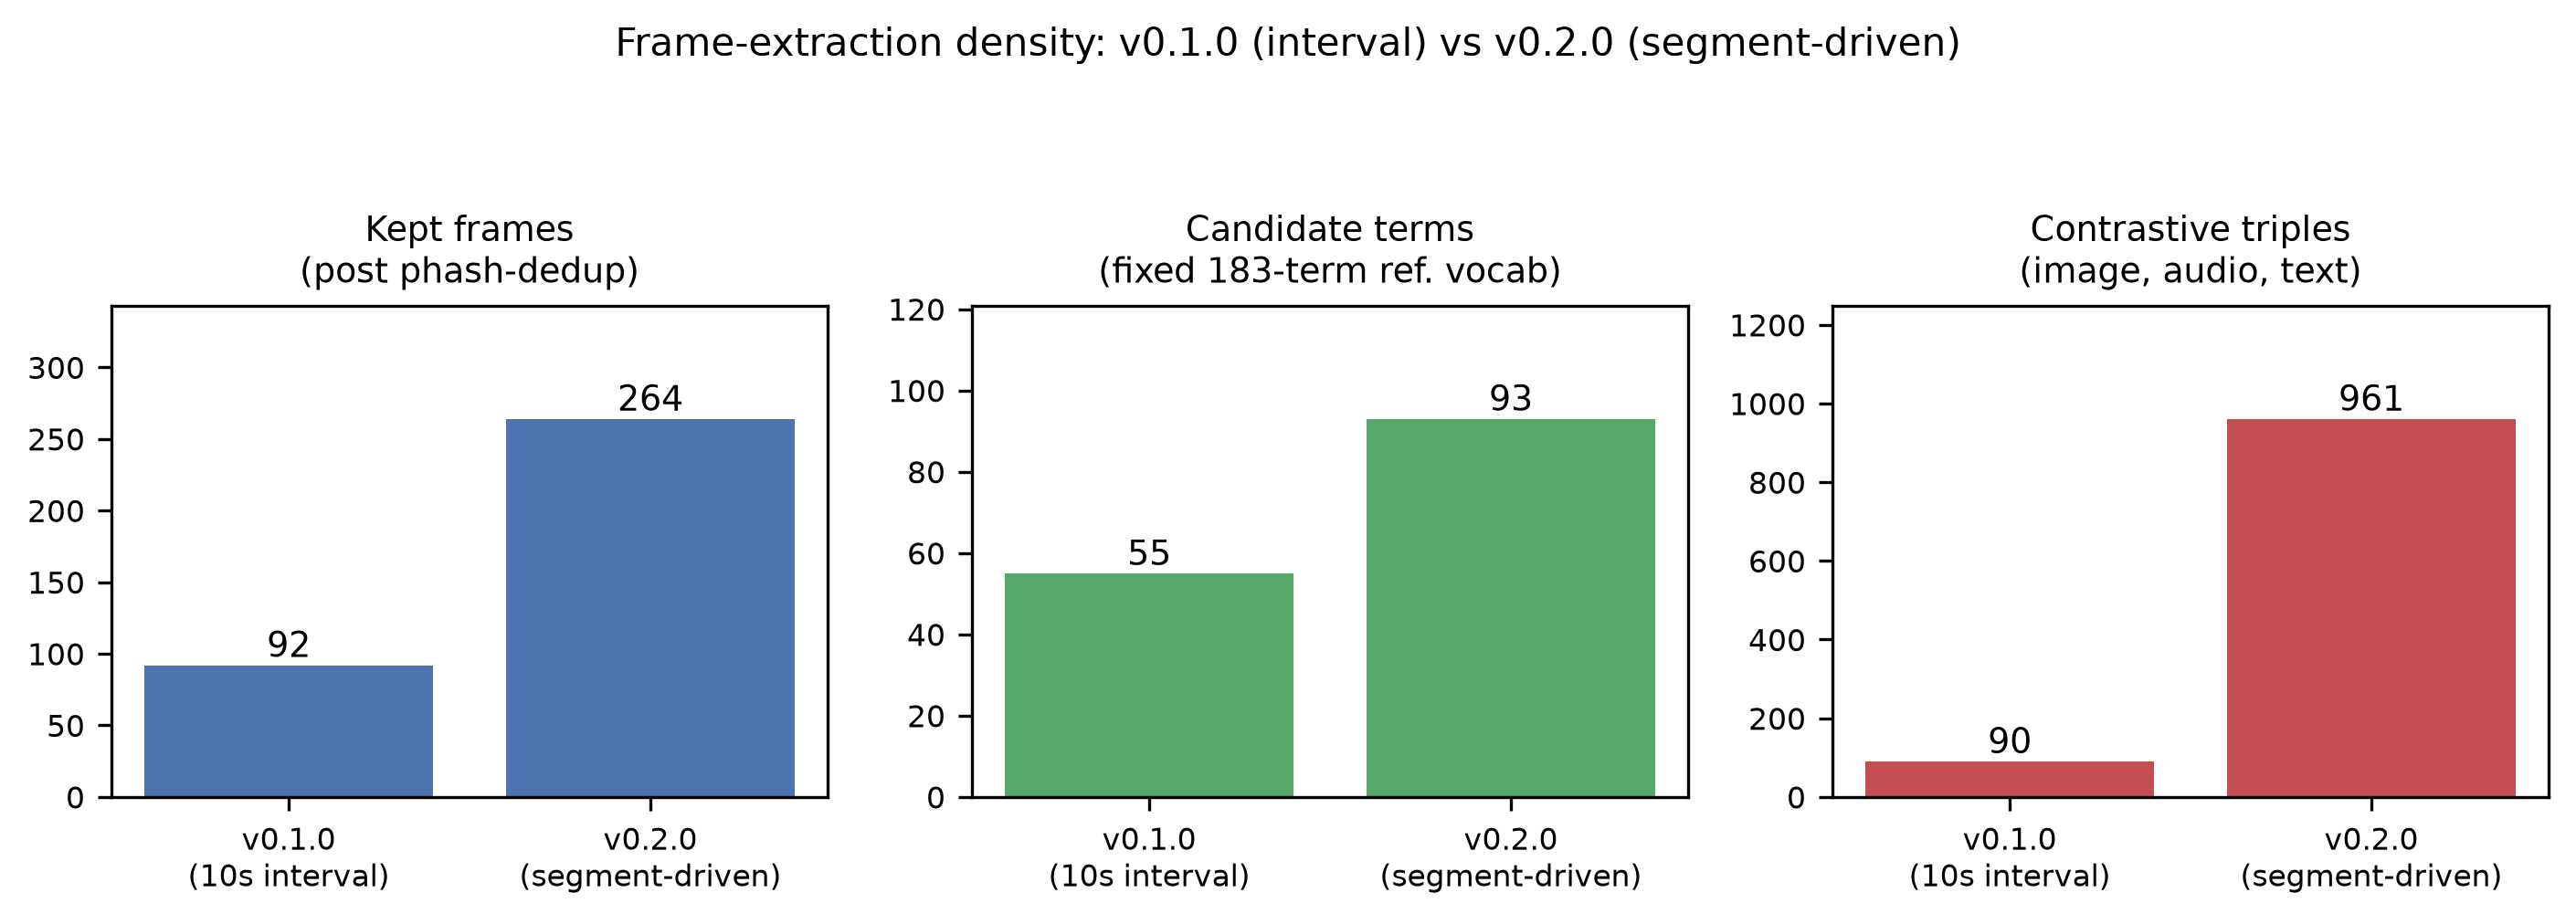
\includegraphics[width=\linewidth]{figures/Fig2_frame_density.png}
\caption{Frame-extraction density and contrastive-triple count, interval ($F_{\text{int}}$) vs.\
segment-driven ($F_{\text{seg}}$) sampling. Candidate-term counts use the fixed 183-term reference
dictionary of \S\ref{sec:setup-protocol}.}
\label{fig:density}
\end{figure*}

\subsection{Dictionary Expansion via Dual Corroboration}

Table~\ref{tab:dictexpand} reports the frame-derived dictionary-expansion outcome across both
sampling strategies, each applied to the \emph{live} dictionary at the time it was run (not the
fixed reference of \S\ref{sec:setup-protocol}, which exists only for the fair method comparison
above). $F_{\text{int}}$'s run merged 29 high-confidence candidates, of which manual audit found 4
to be OCR-artifact false positives (\textit{mama-ateita}, a sentence fragment incorporating the
genuine term \textit{ateita}; \textit{sh\=o-kinbou-kasho}, a truncated form of ``near the bearing
support, location''; \textit{souj\=o-fushoku-No}, a genuine term with a photo-caption numbering
suffix attached; and \textit{kakunin-moku}, a truncated name-fragment collision), leaving 25 genuine
terms merged. $F_{\text{seg}}$'s subsequent run against the now-further-enriched live dictionary
merged 6 additional high-confidence candidates (most of the density gain's genuine new terms,
Table~\ref{tab:framedensity}, had already been captured and excluded as ``known'' by this point), of
which 3 were OCR artifacts caught by the duplication and truncation patterns of
\S\ref{sec:method-frame-import} (\textit{souj\=o-fushoku-No.}, \textit{ji-ry\=o-t\=e-ny\=o}, a
garbled multi-note OCR run; and \textit{souj\=o-fushoku-rikkuru}, a truncated glue artifact),
leaving 3 genuine terms merged (\textit{shiten-bu}, \textit{souj\=o-fushoku}, \textit{anabiki}).
Combined, dual corroboration expanded the dictionary from 183 to 213 entries (+30, of which 28 via
frame OCR across both runs and 2 via the base paper's existing audio-side $E_{\text{meet}}$
mechanism on this same recording, down from the base paper's originally reported 7 since most
candidates it previously discovered post-hoc were already present in the dictionary from this
paper's pre-ASR frame import, \S\ref{sec:discussion}).

\begin{table}[t]
\centering
\caption{Dictionary expansion via frame-derived dual corroboration.}
\label{tab:dictexpand}
\scriptsize
\begin{tabular}{lrrr}
\toprule
Run & Merged & FP (audit) & Net genuine \\
\midrule
$F_{\text{int}}$ (v0.1.0) & 29 & 4 & 25 \\
$F_{\text{seg}}$ (v0.2.0) & 6 & 3 & 3 \\
\midrule
Total frame-derived & 35 & 7 & \textbf{28} \\
Audio-side $E_{\text{meet}}$ & -- & -- & 2 \\
\midrule
Dictionary size & \multicolumn{3}{r}{183 $\rightarrow$ \textbf{213}} \\
\bottomrule
\end{tabular}
\end{table}

\subsection{Contrastive-Triple Density and Training Stability}

Table~\ref{tab:triples} and Figure~\ref{fig:training} report the triple-construction comparison of
\S\ref{sec:method-triples}. Segment-centric construction increases total triples more than tenfold
(90 to 961) while guaranteeing full utterance coverage (914/914 segments, vs.\ 264 frames capping
the frame-centric design's maximum possible triple count); 43 segments contributed more than one
triple because the shared screen changed mid-utterance, a pattern the frame-centric design cannot
represent at all. Figure~\ref{fig:training} shows both training runs' InfoNCE loss: the frame-centric
run (90 triples) converges smoothly to a near-zero loss (13.8 to 0.59 at the best checkpoint),
while the segment-centric run (961 triples) converges to a substantially higher absolute loss (20.75
to 6.62 at the best checkpoint) -- consistent with the larger in-batch negative count raising the
random-chance floor ($\ln 961 \approx 6.87$ per pairwise term) -- and exhibits three distinct
late-training loss spikes (around epochs 140, 320, and 540 of an 800-epoch run) under our fixed
learning rate, which best-checkpoint retention (\S\ref{sec:method-training}) resolves without
requiring a learning-rate schedule.

\begin{table}[t]
\centering
\caption{Contrastive-triple construction: frame-centric vs.\ segment-centric.}
\label{tab:triples}
\scriptsize
\begin{tabular}{lrr}
\toprule
Metric & Frame-centric & Segment-centric \\
\midrule
Total triples & 90 & \textbf{961} \\
Utterance coverage & -- & 914/914 \\
Segments with $>$1 triple & -- & 43 \\
Distinct images reused & -- & 264 \\
Best-ckpt.\ InfoNCE loss & 0.59 & 6.62 \\
\bottomrule
\end{tabular}
\end{table}

\begin{figure}[t]
\centering
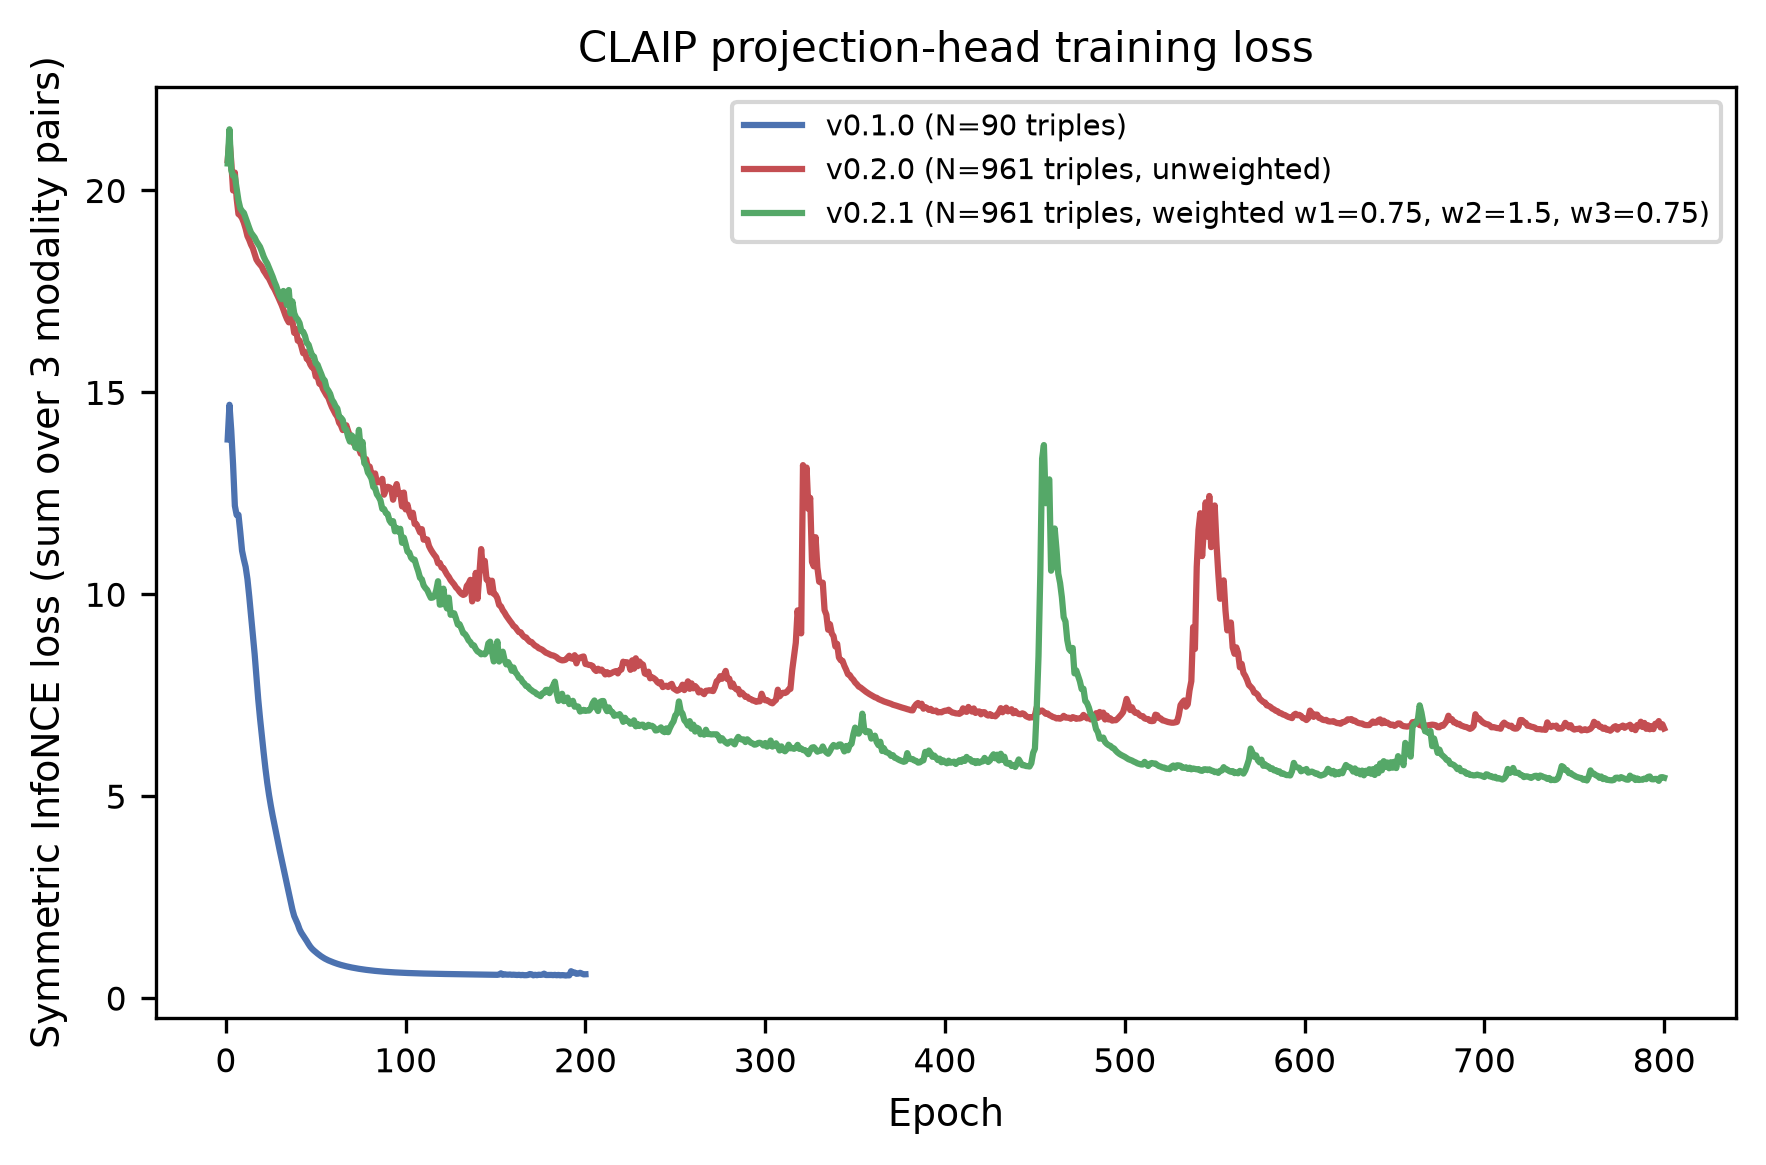
\includegraphics[width=\linewidth]{figures/Fig3_training_curves.png}
\caption{CLAIP projection-head InfoNCE training loss. The segment-centric run's larger in-batch
negative count (961 vs.\ 90 triples) raises both the achievable loss floor and the visible
late-training instability under fixed-learning-rate Adam (\S\ref{sec:discuss-training}). The third
curve (v0.2.1, weighted) is the standby-frame-motivated weighted objective of
\S\ref{sec:results-weighting} ($w_1=0.75, w_2=1.50, w_3=0.75$), trained on the same 961 triples with
the same random seed as a controlled unweighted rerun (not separately plotted here; see
Table~\ref{tab:weighting}).}
\label{fig:training}
\end{figure}

\subsection{Cross-Modal Retrieval Sanity Check}

Figure~\ref{fig:retrieval} reports the 7-query sanity check (\S\ref{sec:setup}). The frame-centric
space (90 triples) correctly retrieves 2 of 7 known domain terms (\textit{aachi-rib},
\textit{hoshuu-houhou}); the segment-centric space (961 triples) correctly retrieves 4 of 7, adding
\textit{ateita} and \textit{shita-flange} while still missing \textit{rivet},
\textit{nakazume}, and \textit{kouzou-keishiki}. We report this as a qualitative, single-recording
proof of concept: with only 7 queries and one video's embedding space, these counts should not be
read as a precisely estimated retrieval accuracy (\S\ref{sec:discussion}).

\begin{figure}[t]
\centering
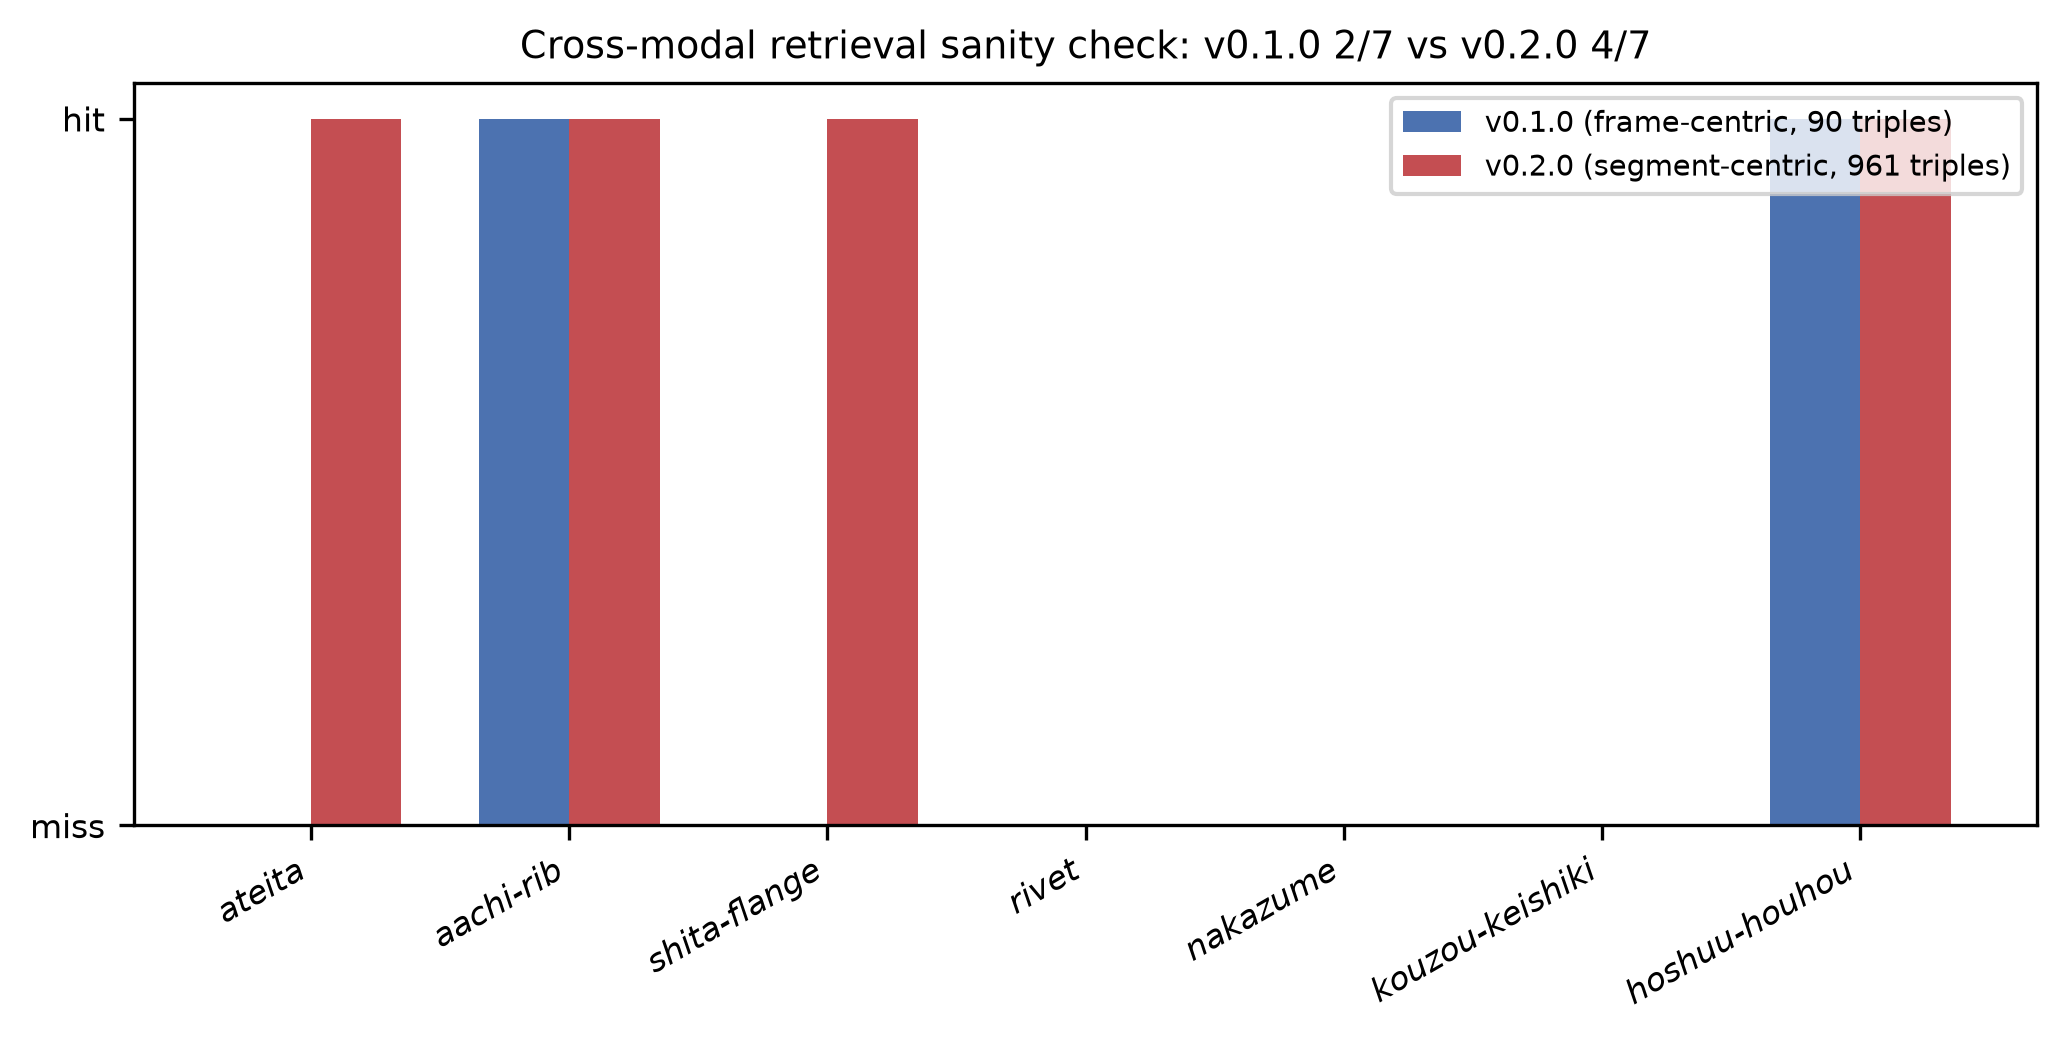
\includegraphics[width=\linewidth]{figures/Fig4_retrieval_hitrate.png}
\caption{Cross-modal retrieval sanity check, 7 known high-confidence domain terms (romanized).
Segment-centric training (961 triples) nearly doubles the hit rate observed with frame-centric
training (90 triples).}
\label{fig:retrieval}
\end{figure}

\subsection{Loss Weighting for the Standby-Frame Hypothesis}
\label{sec:results-weighting}

To test whether the per-pair loss weighting motivated in \S\ref{sec:method-training} is actually
beneficial, we trained two projection heads on the same 961 segment-centric triples with a fixed
random seed (so the two runs differ only in $w_1, w_2, w_3$, not in initialization): an unweighted
control ($w_1=w_2=w_3=1$) and a hand-chosen weighted setting ($w_1=0.75$, $w_2=1.50$, $w_3=0.75$,
summing to the same total weight as the unweighted case). Table~\ref{tab:weighting} reports the
outcome. The weighted run reaches a lower best-checkpoint loss (5.38 vs.\ 6.69) and shows one
late-training loss-spike event instead of two over the same 800 epochs (Figure~\ref{fig:training}).
Because $w_1, w_3 < 1 < w_2$ changes the objective's nominal scale, we additionally re-scored both
runs' best checkpoints under the common, \emph{unweighted} sum $\mathcal{L}_{\text{NCE}}(\text{img},
\text{txt}) + \mathcal{L}_{\text{NCE}}(\text{aud},\text{txt}) + \mathcal{L}_{\text{NCE}}(\text{img},
\text{aud})$ to separate a genuine per-pair improvement from this scale effect: on this common
footing, the audio-text pair improves by 19.8\% (0.803 to 0.644), while the image-text and
image-audio pairs are essentially unchanged (within 1.5\%, i.e.\ not measurably degraded despite
their lower weight). The 7-query retrieval hit rate (\S\ref{sec:setup}) is unchanged at 4/7 for both
runs.

\begin{table*}[t]
\centering
\caption{Standby-frame-motivated loss weighting: seed-matched unweighted vs.\ weighted
($w_1=0.75, w_2=1.50, w_3=0.75$), same 961 triples.}
\label{tab:weighting}
\scriptsize
\begin{tabular}{lrrr}
\toprule
Metric & Unweighted & Weighted & $\Delta$ \\
\midrule
Best-ckpt.\ loss (as trained) & 6.69 & \textbf{5.38} & -19.6\% \\
Final-epoch loss & 7.08 & \textbf{5.46} & -22.9\% \\
Late-training spike events & 2 & \textbf{1} & -- \\
\midrule
\multicolumn{4}{l}{\textit{Per-pair loss, re-scored unweighted (common basis):}} \\
\ \ image-text & 2.936 & 2.979 & +1.5\% \\
\ \ audio-text & 0.803 & \textbf{0.644} & \textbf{-19.8\%} \\
\ \ image-audio & 2.996 & 3.020 & +0.8\% \\
\midrule
Retrieval hit rate (7 queries) & 4/7 & 4/7 & -- \\
\bottomrule
\end{tabular}
\end{table*}

%% ====================================================================
\section{Discussion}
\label{sec:discussion}
%% ====================================================================

\subsection{Why Utterance-Aligned Sampling Density Matters}

The base paper's processing-time analysis found that per-segment invocation overhead means
high-turn-density meetings cost disproportionately more to process; this paper's frame-density
results generalize the same underlying principle from \emph{cost} to \emph{coverage}: sampling at a
granularity tied to the unit of downstream analysis (the diarized utterance) rather than an
arbitrary wall-clock interval recovers more of the content that matters for that analysis, whether
the cost being optimized is processing time (base paper) or candidate-term/training-data coverage
(this paper). A fixed interval is both too coarse (slide transitions between sample points are
simply missed, \S\ref{sec:method-frames}) and too indiscriminate (many redundant samples of an
unchanging slide, later discarded by de-duplication) relative to sampling that follows the audio's
own segmentation.

\subsection{A Third Candidate-Extraction Failure-Mode Family}
\label{sec:discuss-ocr}

The base paper reports two distinct audio-side candidate-extraction failure-mode families: naive
substring collision at the morphological level, and LLM topical-relevance misjudgment at the
semantic level. This paper's two OCR-specific failure modes
(\S\ref{sec:method-frame-import}) constitute a third family, arising neither from Japanese
morphology nor from LLM judgment, but from OCR text's complete lack of natural-language structure
(no word boundaries where there would be whitespace in a Western script, no particles, no sentence
punctuation separating visually adjacent but semantically unrelated screen content). The
generalizable lesson across all three families is the same as the base paper's for morphology
specifically: \emph{any} automated vocabulary-candidate-extraction mechanism must be audited against
the specific structural properties of its actual input text, not assumed safe merely because a
similar mechanism worked safely on a different text source (audio transcript vs.\ external ontology
vs., now, OCR). Notably, the proportion of false positives among frame-derived merges (7 of 35, 20\%)
is substantially lower than the base paper's reported audio-side per-meeting false-positive rate
before mitigation (11 of 14, 79\%, on an earlier meeting, improving to 0 of 7 only after four
dedicated mitigations) -- consistent with frame OCR's candidates being exact, verbatim written text
rather than a speech-recognition hypothesis layered on top of an acoustic model's own uncertainty,
even though OCR introduces its own distinct noise sources.

\subsection{Training Stability at Increased Triple Count}
\label{sec:discuss-training}

The qualitative difference between the two training curves in Figure~\ref{fig:training} --
monotonic near-convergence at 90 triples versus a higher loss floor with intermittent spikes at 961
-- is, to our knowledge, not previously reported for this small-scale, single-recording contrastive
training regime, where triple count is set entirely by how one real meeting's content happens to be
structured rather than by a deliberately chosen dataset size. We attribute the increased instability
to the larger in-batch negative count interacting with a fixed learning rate under full-batch Adam
(no mini-batching, since all triples fit in GPU memory): as the embedding space sharpens, a given
gradient step can more easily overshoot a now-narrower optimum, producing the isolated spikes
visible in Figure~\ref{fig:training} around epochs 140, 320, and 540. Best-checkpoint retention is a
minimal, zero-additional-hyperparameter mitigation; we did not evaluate whether a learning-rate
schedule would avoid the spikes altogether, or whether they recur at a different triple count,
and flag both as natural next steps once multi-recording training (\S\ref{sec:conclusion}) makes
mini-batching necessary regardless.

\subsection{Loss Weighting Mitigates Training Instability, but Mostly via Audio-Text}
\label{sec:discuss-weighting}

The weighted run's lower raw loss and halved spike count (\S\ref{sec:results-weighting}) might at
first look like a general sharpening of the shared embedding space, but the per-pair re-scoring in
Table~\ref{tab:weighting} shows this is not quite the right reading: nearly all of the measured
improvement is concentrated in the audio-text pair, the one pair we up-weighted ($w_2=1.50$) and
whose hypothesis-driven motivation (\S\ref{sec:method-training}) was precisely that it should remain
reliable even when a frame is uninformative. The two down-weighted, image-involving pairs
($w_1=w_3=0.75$) are not degraded, but neither do they improve -- they are, as expected, simply
getting slightly less gradient signal per step. We read this as mild, directionally consistent
support for the standby-frame hypothesis (up-weighting the modality pair least affected by an
uninformative image does help that pair, without visibly harming the others) rather than evidence
that this specific weight choice meaningfully improves the trained space's overall cross-modal
alignment: the unchanged 4/7 retrieval hit rate (Table~\ref{tab:weighting}) is consistent with this
more modest interpretation. A sharper test of the hypothesis would require first measuring how many
triples in a recording actually contain a standby frame (not done here, \S\ref{sec:discuss-ocr}) and
comparing weighted training with and without those specific triples present, rather than applying a
single hand-chosen weight triple uniformly to all 961 triples regardless of whether each one's image
is a standby tile.

\subsection{Limitations}

We report the following limitations candidly, extending the base paper's own Limitations
subsection. First, both the frame-extraction-method comparison and the CLAIP training/retrieval
results are a \emph{single-recording} case study; the dictionary-expansion false-positive rates and
training-stability observations of \S\ref{sec:discuss-ocr}--\S\ref{sec:discuss-training} are
informative single-instance evidence, not statistically estimated rates, matching the base paper's
own small-sample caveat for its audio-side dictionary-expansion evaluation. Second, the 7-query
retrieval sanity check (\S\ref{sec:results}) uses a closed, 264-to-961-row candidate set drawn from
the same single recording it was trained on; it demonstrates that the mechanism functions as
designed, not a generalizable retrieval accuracy, and future work should evaluate on a held-out
recording once multiple recordings are available. Third, the sub-sampling interval ($\tau=3.0$\,s)
and per-segment cap ($K=5$) in Equation~\ref{eq:k-samples} are empirical choices tuned to this
recording's statistics (median segment duration 1.43\,s) and untested on meetings with
substantially different speech-turn or screen-share-change cadence. Fourth, the external
\texttt{rinnakk/japanese-clip} repository referenced by the model's own documentation was
unavailable (HTTP 404) at the time of this work, requiring us to install an alternative community
fork and apply two compatibility patches for API drift against current \texttt{transformers}/
\texttt{huggingface\_hub} releases; this is a reproducibility risk inherent to depending on an
actively-evolving third-party ecosystem rather than a methodological limitation of the approach
itself, but future replications should expect to re-verify this dependency chain. Fifth, the
InfoNCE temperature ($\tau_{\text{nce}}=0.07$), projection dimensionality (256), and training-epoch
budget (800 for the segment-centric run) were fixed by convention rather than tuned via a
hyperparameter sweep. Sixth, the loss-weighting ablation (\S\ref{sec:results-weighting}) tests a
single hand-chosen weight triple on a single recording with a single random seed; we did not sweep
$w_1, w_2, w_3$ systematically, nor did we measure how many of the 961 triples' frames are actually
standby tiles (\S\ref{sec:discuss-weighting}), so we cannot attribute the observed audio-text
improvement specifically to standby frames being down-weighted versus a more general effect of
shifting relative pair weights; detecting standby frames automatically (e.g., from their
near-uniform black background) and comparing training with and without them present is a
prerequisite for a more direct test of the hypothesis.

\subsection{Practical Implications}

For practitioners, the central practical finding is that \emph{how} a fixed amount of screen-share
video is sampled matters as much as \emph{whether} it is used at all: aligning frame sampling to the
same utterance segmentation already computed for diarization, rather than an independent wall-clock
interval, is a low-cost change (no additional model, only a different set of \texttt{ffmpeg} seek
timestamps) that measurably improves both dictionary-expansion coverage and contrastive-training
data density. The dual-corroboration mechanism (\S\ref{sec:method-frame-import}) further lets an
organization's own in-meeting screen content -- design drawings, inspection photographs,
sticky-note review annotations -- directly improve same-run ASR vocabulary bias, requiring no
external knowledge source beyond the recording itself, complementary to the base paper's
ontology-corroborated bulk import.

%% ====================================================================
\section{Conclusion}
\label{sec:conclusion}
%% ====================================================================

\subsection{Concluding Remarks}

We extended an on-premise construction-meeting ASR pipeline's dictionary-correction mechanism with
a second, independent corroboration source -- screen-share frame OCR, available before speech
recognition runs -- and built a three-modality shared embedding space via CLAIP-style contrastive
learning over the same recording's own utterance-aligned data. Our central empirical finding is
that aligning frame sampling to the diarization segmentation already computed for ASR, rather than
sampling at a fixed wall-clock interval, substantially improves both candidate-term coverage (+69\%
under a controlled, fixed-reference-vocabulary comparison) and contrastive-training data density
(90 to 961 triples, full utterance coverage), which together nearly double a qualitative cross-modal
retrieval sanity check (2/7 to 4/7). We additionally reported a third family of candidate-extraction
failure modes specific to OCR text, and an empirical contrastive-training-stability finding as
triple count scales by an order of magnitude on a single recording. Motivated by the standby-frame
case -- a Google Meet participant tile entering a triple in place of genuine shared-screen content
-- we introduced a per-modality-pair loss weighting and, in a seed-matched ablation, found that one
hand-chosen weighted setting sharpens the audio-text pair substantially (-19.8\%) without degrading
the image-paired terms and roughly halves the observed late-training spike count, though it leaves
the qualitative retrieval hit rate unchanged -- a safe but modest refinement on this evidence, not a
demonstrated fix. As with the base paper, we
report all results candidly, including a single-recording case study's inherent limitations
(\S\ref{sec:discussion}).

\subsection{Future Work}

In the near term, we plan to (i) extend this evaluation to multiple recordings, both to obtain
statistically meaningful dictionary-expansion false-positive rates and retrieval accuracy
(\S\ref{sec:discussion}) and to make mini-batched, learning-rate-scheduled contrastive training
necessary and evaluable (\S\ref{sec:discuss-training}); (ii) crop the shared-screen region of a
frame before computing its perceptual hash, rather than hashing the full frame including the
Google Meet participant-gallery tile, to test whether de-duplication becomes more precise;
(iii) evaluate a learning-rate schedule (warmup/decay) as an alternative or complement to
best-checkpoint retention; and (iv) detect standby frames automatically (e.g., a near-uniform
black background with a single centered name/photo tile), measure their actual frequency among the
961 triples, and use that detector to compare training with and without the affected triples
present, or to sweep Equation~\ref{eq:weighted-infonce}'s per-pair weights $w_1, w_2, w_3$ across
multiple seeds and settings rather than the single hand-chosen triple evaluated in
\S\ref{sec:results-weighting}, so that any further gain can be attributed specifically to standby
frames rather than to a general shift in relative pair weights. Beyond these near-term items, this extension is a direct step toward the
project's own Concept Note vision of CLAIP-based cross-modal meeting search: with a trained shared
embedding space in place, a natural next step is a query interface over the corroborated
vector store -- e.g., FAISS-indexed nearest-neighbor search over
$\pi_{\text{img}}, \pi_{\text{aud}}, \pi_{\text{txt}}$ projections -- letting an engineer search a
meeting archive by natural-language query across audio, screen content, and text simultaneously.
More broadly, the dual-corroboration principle demonstrated here -- that an organization's own
in-meeting artifacts (here, screen-share content) can directly verify and expand a domain dictionary
without depending solely on an external knowledge source -- suggests further independent evidence
sources worth corroborating against in future work, such as shared design documents or chat logs
exchanged during the same meeting, extending the same dual-corroboration mechanism to additional
in-meeting modalities beyond audio and screen-share video.

Looking further ahead, this bridge-repair design-review case study is best read as a first domain
instance of the broader Meeting Intelligence goal introduced in \S\ref{sec:intro}: using an
organization's own meeting video, rather than an external corpus, as the raw material for
continuously corroborated, specialized-domain ontology construction. Having validated the
dual-corroboration and segment-aligned contrastive-triple mechanisms within one construction
sub-discipline (bridge structural repair), a natural cross-sectional extension is to the many other
specialized engineering departments an infrastructure-services organization such as ours maintains
across the broader construction field -- roads and railways, rivers/dams and erosion control
(\textit{sabo}), architecture and parks, and environment/energy -- each with its own damage-cause
vocabulary, review-meeting conventions, and screen-share artifact types, but sharing the same
underlying pipeline. We envision this domain adaptation as populating an agentic
mesh~\cite{debnath2025agenticmesh} of department-specific ontology-corroboration and retrieval
agents, each independently verified against its own domain evidence yet interoperable through a
shared CLAIP-style embedding space and cross-domain workflow-composition
mechanisms~\cite{wang2026crossdomainworkflow}, so that a query spanning multiple specialized
departments (e.g., a river-crossing bridge repair touching both structural and hydraulic domains)
can be routed to, and corroborated by, the relevant department-specific agents without re-deriving a
shared ontology from scratch.

\bibliographystyle{unsrt}
\bibliography{meet_mp4_claip_2026}

\end{document}


